\section{Methods}
\label{sec:Methodes}


The optimization of the films was formulated as finding the minimum mass of \iso[6]{Li} for a given detector material necessary to fulfill an interaction rate of \SI{2.5}{cps\per\nano\gram\iso[252]{Cf}} while maintaining a intrinsic gamma rejection ratio of \num{1.e-6}.

It is assumed that there is a fixed cost to assemble each detector assembly and mount it between the moderator.

\todo[inline]{Cost Trade-off section. In detector designs there can never be too much reflector based on a neutronics perspective, however at some point the moderator serves to reflect neutrons back to the source.}

\subsection{Design Parameters}
\label{sec:DesignParameters}
The design parameters were then:
\begin{itemize}
  \item The detector material. Materials with a high \iso{6}[Li] concentration will absorb more neutrons.
  \item The thickness of the detector material.
  \item The spacing of detector layers.
  \item The initial moderator thickness.
\end{itemize}

The geometry is described as follows:
There is an initial moderator of \SI{2.5}{\centi \meter} HDPE to achieve a thermal fraction around 10\%.
\footnote{The thermal energy was chosen to be \SI{5}{\electronvolt}. 
The \isotope[6]{Li} neutron cross section as this energy is 67 barns. 
A sample containing 10\% \iso[6]{Li} and a density of\SI{1.0}{\gram \per \cubic \centi\meter} would then macroscopic cross section of \SI{0.67}{\per \centi\meter}, attenuating \SI{0.67}{\percent} of the incident flux in \SI{0.01}{ \centi\meter}. 
The macroscopic cross section calculation is shown below. 
\begin{align*}
\Sigma &= \frac{\rho N_A}{M}  \left ( n_1 \sigma_1 + n_2 \sigma_2 + n_3 \sigma_3 + \dots  \right ) \\ 
       &= \frac{\rho N_A n_1 \sigma_1}{M} \\
       &= \frac{\SI{1.0}{\gram\per\cubic\centi\meter} \SI{6.022E23}{\per\mole} \SI{67}{\barn}{0.05}}{6} \\
       &= \SI{0.67}{\per\centi\meter} 
\end{align*}
}..
Following the moderator there are repeated sections of detector assembly and moderator.
A single detector assembly consists of a layered film \SI{100}{\micron} thick with a light guide of \SI{0.5}{\centi\meter}.
After the absorb film and light guide assemblies is additional moderator.
Four basic detector designs were considered, as shown in Figure ~\ref{fig:OptDesignSchematics}
In the first design there are only three parameters; the thickness of the moderator $P_1$, the thickness of the reflector $P_2$ and the number of layers, $n$. 
In the second detector design (B) there are two assemblies of layered detectors surrounded by HDPE moderator.  Thus there are five parameters to optimize; the thickness of the front moderator $p_1$, the thickness of the moderator separating the assemblies $p_2$, the thickness of the reflector $p_3$, and the number of films in each assembly, $n_1$ and $n_2$.
Similarly there are seven parameters to optimize in design C, and nine parameters to optimize in design D.

\begin{figure}
    \centering
    \begin{subfigure}[b]{0.45\textwidth}
        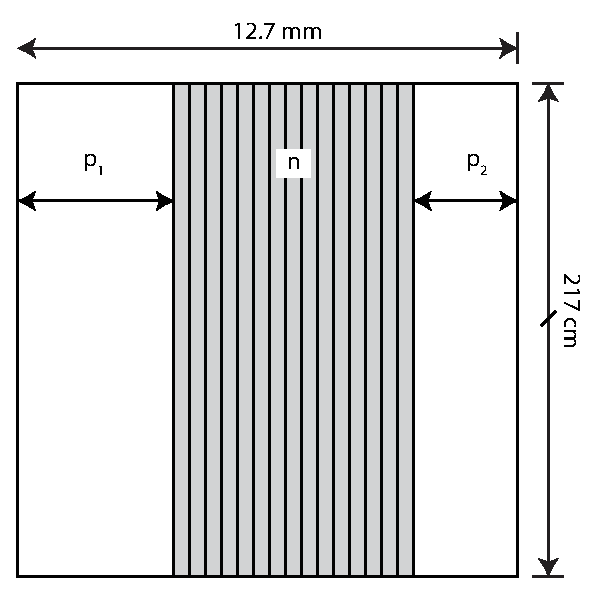
\includegraphics[width=\textwidth]{RPM8_Diagrams_OptDesign_A}
        \caption{A single detector assembly}
    \end{subfigure}
    ~
    \begin{subfigure}[b]{0.45\textwidth}
        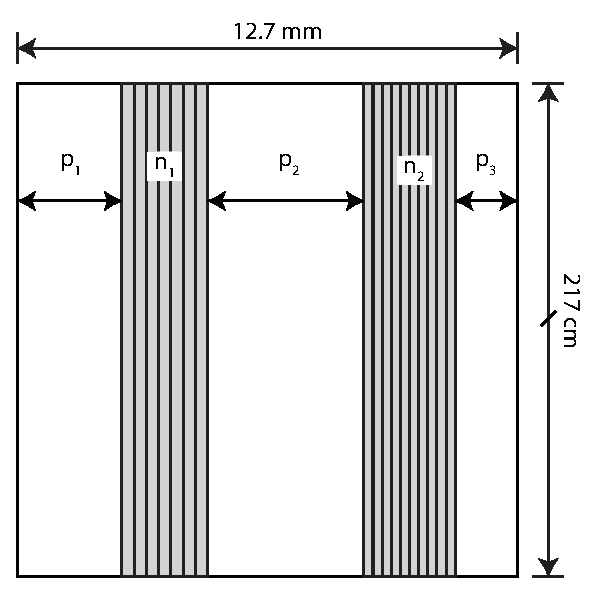
\includegraphics[width=\textwidth]{RPM8_Diagrams_OptDesign_B}
        \caption{Two detector assemblies}
    \end{subfigure}

    \begin{subfigure}[b]{0.45\textwidth}
        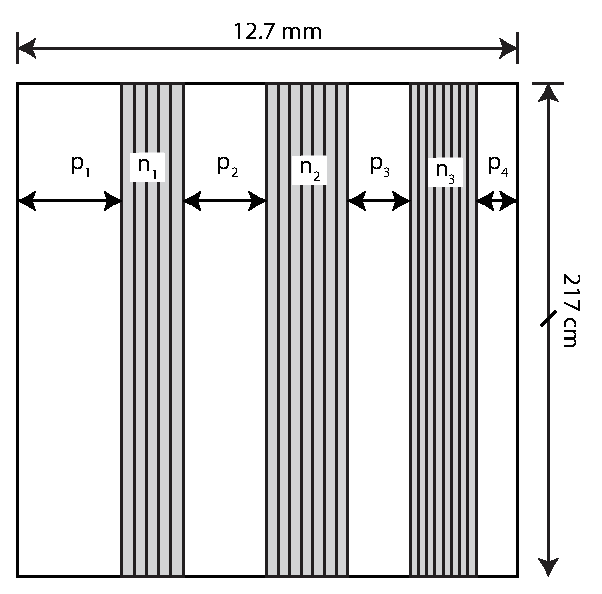
\includegraphics[width=\textwidth]{RPM8_Diagrams_OptDesign_C}
        \caption{Three detector assemblies}
    \end{subfigure}
    ~
    \begin{subfigure}[b]{0.45\textwidth}
        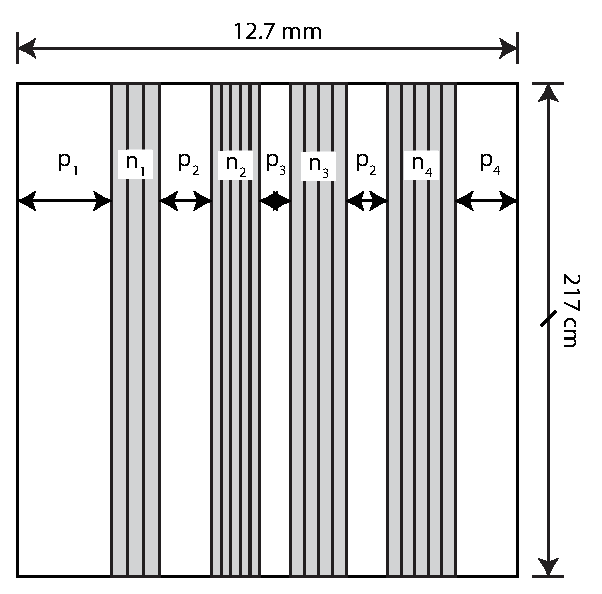
\includegraphics[width=\textwidth]{RPM8_Diagrams_OptDesign_D}
        \caption{Four detector assemblies}
    \end{subfigure}
    \caption{Detector Designs for Optimization}
    \label{fig:OptDesignSchematics}
\end{figure}

Figure ~\ref{fig:MCNPXRendering} shows the MCNPX renderings of the X-Z profile of two detector configurations.
The source is not shown as it is located \SI{2}{\meter} from the detector midpoint.

\begin{figure}
    \centering
    \begin{subfigure}[b]{0.45\textwidth}
        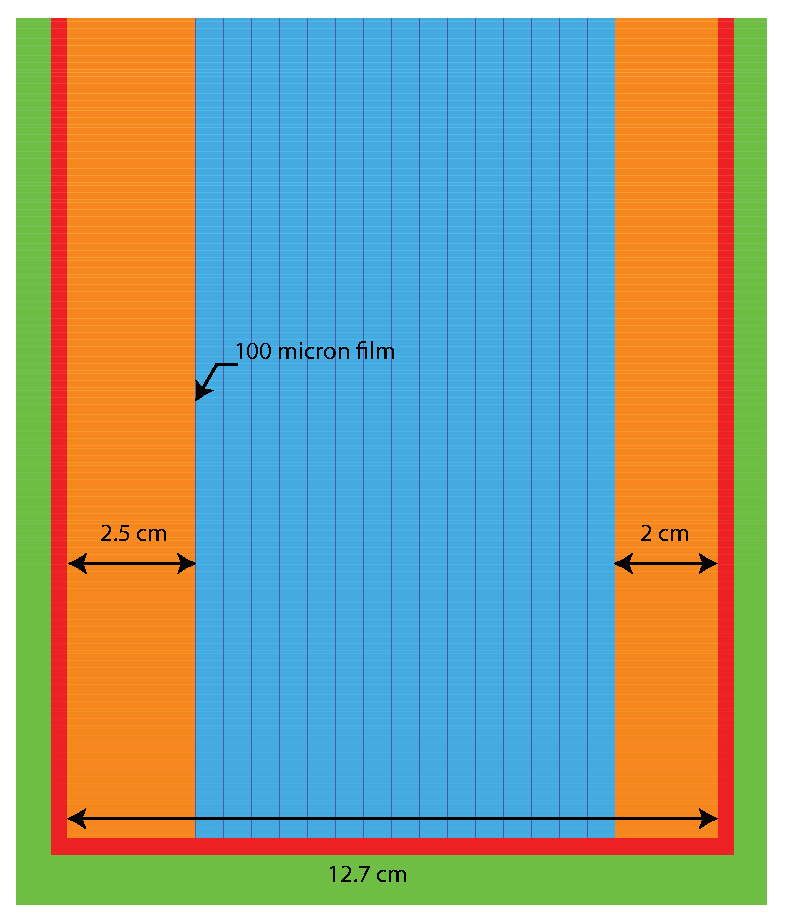
\includegraphics[width=\textwidth]{RPM8_Diagrams_MCNPXRender_1Assm}
        \caption{MCNPX Model of One Assembly}
    \end{subfigure}%
    ~
    \begin{subfigure}[b]{0.45\textwidth}
        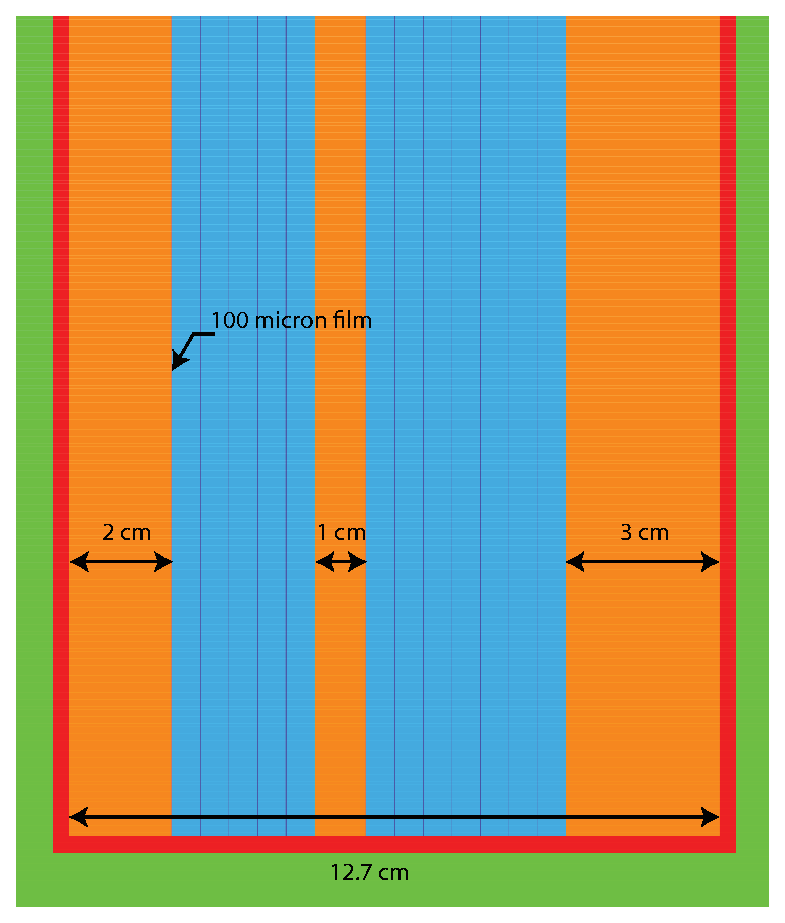
\includegraphics[width=\textwidth]{RPM8_Diagrams_MCNPXRender_2Assm}
        \caption{MCNPX Model of Two Assemblies}
    \end{subfigure}
    \caption{MCNPX rendering of layered geometry}
    \label{fig:MCNPXRendering}
\end{figure}
The optimization of the detector design is presented in two parts: a numerical approach in which a matrix of detector spacing and assemblies are varied (Section ~\ref{sec:MCNPXMethods}, and a multivariate-variate optimization in which the parameters are fit to a functional form which is then optimized (Section ~\ref{sec:MVOptimization}).
\subsection{MCNPX Simulations}
\label{sec:MCNPXMethods}
A matrix of detector designs was simulated in MCNPX, with the parameters are described in Table \ref{tab:MCNPXGeoMatrix}.
A generic script file was written (Listing ~\ref{lst:MCNPScript}) that was modified with the code in Listing ~\ref{lst:CreateSurfaceCell} to include a user supplied number of detector assemblies, spacing between these assemblies, and initial moderator at the front of the assembly.
The MCNPX output was post processed with the python modules presented in Listing ~\ref{lst:ParseOutput} and Listing ~\ref{lst:mctal}.
See ~\ref{sec:RPM8Listings} for detailed information on the developed scripts and details on the running of the problems.
\begin{table}
	\caption{Number of Film Assemblies and Spacing of MCNPX Simulations}
	\label{tab:MCNPXGeoMatrix}
  \centering
	\input{MCNPXGeoMatrix.dat}
\end{table}

Two tallies were used in the MCNPX calculations: the interaction rate tally (tally type 4) and the surface flux tally (type 2).
If the scalar flux is defined as $\phi(\vec{r},E,t)=\int d\Omega \Phi(\vec{r},\hat{\Omega},E,t)$ the  interaction rate tally is the integral of all energies and directions of the scalar flux over a given volume, normalized by that volume ~\eqref{eqn:F4TallyDef}.
This quantity is then modified by an FM card which calculates quantities of the form $Q = C \int {\Phi(E) R_m(E) dE }$ where:
\begin{itemize}
    \item $C$ is a scalar normalization (density)
    \item $R_m(E)$ is the response function
    \item $\Phi(E)$ is the neutron flux
\end{itemize}
Similarly the surface flux is the integral over the entire surface (normalized by the surface area) of the scalar flux, as shown in \eqref{eqn:F2TallyDef}.
\begin{align}
    \label{eqn:F4TallyDef}
    \bar{\phi_V} = \frac{1}{V}\int dE \int dt \int dV \int d\Omega \AngularFlux
\end{align}
\begin{align}
    \label{eqn:F2TallyDef}
    \bar{\phi_S} = \frac{1}{A}\int dE \int dt \int dA \int d\Omega \AngularFlux
\end{align}

The FM card can modify any flux or current tally of the form $\int \psi (E) dE$ into $\int R(E)\psi(E) dE$, where $R(E)$ is the response function known to MCNP.
\subsection{1 D Transport Part}
The large detector and far away source suggest that the problem can be simplified into a one dimensional transport problem without suffering the accuracy of the solution.
As 1D deterministic transport is much faster than 3D Monte Carlo, 1D transport was explored in order to vary the problem parameters.

A matrix of \SI{25}{\percent} \iso[6]{Li} PEN films were completed with the film assemblies being 1,2,3, and 4 and with a spacing of \SI{1}{\centi\meter},\SI{2}{\centi\meter},\SI{3}{\centi\meter},and \SI{4}{\centi\meter}. 


\subsection{Multivariate Optimization}
\label{sec:MVOptimization}

The multivariate optimization problem was formulated as finding $\min_{\vec{x}} f (\vec{x})$ subject to constraints, where $f(\vec{x})$ is the response function.

\subsubsection{Genetic Algorithm}
\label{sec:GeneticAlgoMethods}
Genetic algorthims provide a search method analous to biological evoluation.
Rather than following a gradient of a response function, genetic algorthims generate possible hypothesis by repeatably applying genetic operators (mutation and recombination) of the best currently known hypothesis in order to generate new ones\todo{CIte Mitchel}.
In this way the search space of canidate hypothesis (possible detector designs) is searched to identify the best hypothesis; the design that uses the least amount of \iso[6]{Li} while meeting the critera.
The genetic algorithm typically consist of four tasks: creating an initial population, evaluating that populations fitness, selecting members of the current population to breed, and then applying genetic operators to the selected members to breed the new population. 
This is completed for either a maximum generation is reached or the desired fitness is achieved. 

\begin{figure}
\begin{algorithmic}
  \WHILE{$error>goal$}
		\FORALL{$p \in P$}
			\STATE{Compute fitness}
		\ENDFOR
		\FORALL{$p \in P$}	
			\STATE{Choose individuals based on fitness}
			\STATE{Select individuals for next population}
			\STATE{Crossover selected individuals}
			\STATE{Mutate selected individual}
		\ENDFOR
	\ENDWHILE
\end{algorithmic}
\caption{Genetic Program Outline}
\label{AlgoOutline}
\end{figure}

The genome representation of the geometry was chosen to be represented as a bit string.
Each \verb+1+ or \verb+0+ in the string would represent a detector slice or a moderator slice, respectively.
For example the sequence \verb+0001110010+ would represent a detector that had three moderator slices, three detector slices, another two moderator slices, and a final detector slice before a single moderator slice as the reflector.
It was originally thought to have all of the moderator and detector slice the same thickness, \SI{0.5}{\centi \meter}\footnote{Astute readers may note that with a \SI{0.5}{\centi \meter} light guide and \SI{100}{\micro \meter} detector that the detector size is not \SI{0.5}{\centi\meter} and that 25 slices of \SI{0.5}{\centi\meter} each is \SI{0.2}{\centi\meter} short of the RPM8 size. However, it is not envisioned that \SI{20}{\milli\meter} will greatly impact the solution, or be within the manufacturing tolerances. }.
However, that would create 25 slices with a search space of $2^{25}$ or 33.5 million options.

\todo[inline]{A possibility would be to do a 2 centimeter reflector and a 2 centimeter reflector as constant.  This would then only have $2^{15}$ options, 32,000. I don't want to mess with different sized layers, because then my genomes are different lengths, and it becomes difficult to ensure that it is a correct geometry}.

The fitness function was choosen to count rate per mass of \iso[6]{Li}.
\todo[inline]{Implmeneation of the fitness function might be completed by a dictionary of precomputed geometries. Interlopation could then be used to calculate the interaction of new geometries, and these could then be added to the dictionary.  An ANN might be used for the interoplation, and then retrained (or maybe online training) after a certain number of new hypothesis are made.  It might be useful to have some sort of degree of similarity between hypothsis. One might be logical and of the two hypothesis. In this case 0 would be the same, and len(hypothesis) would be the most disimilar.  Maybe if they are greater than 25 percent different we would want to run the case and add it?}
